\chapter{Methodology}

To create a mathematical foundation for the calculations, it makes sense to explain the theory behind the scrips and programs used for the simulations. A detailed explanation would be extensive, and the explanations will therefore be kept relatively short. The goal is that a reader with sufficient knowledge within the field can refresh their theory and create an intuition on how it is applied. 


%%%%%%%%%%%%%%%%%%%%%%%%%%%%%%%%%%%%%%%%%%%%%%%%%%%%%%%%%%%%%%%%%%%%%%%%%%%%%%%
\section{CFD}
To compute power output and loads on the turbines, it is essential to know how the air behaves around the turbine. Derived from Newtons 2. law, the Navier-Stokes equations can describe movements within the fluid

\begin{equation}
\rho \frac{D u}{D t}=-\nabla p+\nu \nabla^2 u+F,
\label{navier}
\end{equation}
\begin{equation}
    \nabla \cdot u=0,
\end{equation}

where $u$ is velocity, $p$ is pressure, $\mu$ is viscosity and $S$ is external body forces. These equations are complicated to calculate analytically due to the nonlinearity, and solving these numerically for different input parameters is necessary. The simulations are performed in EllipSys3D \cite{ellipsys}, a program utilising high-fidelity Large Eddy Simulations (LES). The program allows us to input different turbine configurations and outputs the behaviour of the wake in a time interval.


%%%%%%%%%%%%%%%%%%%%%%%%%%%%%%%%%%%%%%%%%%%%%%%%%%%%%%%%%%%%%%%%%%%%
\subsection{Large Eddy Simulation}
\label{sec:LES}

In broad terms, LES \cite{LES} is a method within CFD that allows us to filter out small energy eddies, drastically reducing computational time. This is achieved by introducing a filter defined by

\begin{equation}
    \boldsymbol{u}(\boldsymbol{x}, t)=\overline{\boldsymbol{u}}(\boldsymbol{x}, t)+\boldsymbol{u}^{\prime}(\boldsymbol{x}, t), \quad \overline{\boldsymbol{u}}(\boldsymbol{x}, t)=\int G(\boldsymbol{\epsilon} , \boldsymbol{\Delta}) \boldsymbol{u}(\boldsymbol{x}-\boldsymbol{\epsilon}, t) \boldsymbol{d} \boldsymbol{\epsilon},
\end{equation}

where $\Bar{u}$ is the spatial mean and $u^\prime$ is the fluctuations. Applying this to the Navier Stokes equation \ref{navier} yields

\begin{equation}
    \frac{\partial \bar{u}_j}{\partial t}+\frac{\partial \overline{u_i u_j}}{\partial x_i}=-\frac{1}{\rho} \frac{\partial \bar{p}}{\partial x_j}+\frac{\partial}{\partial x_i}\left(\nu\left(\frac{\partial \bar{u}_j}{\partial x_i}+\frac{\partial \bar{u}_i}{\partial x_j}\right)\right)+\bar{F}_j
    \label{filterednavier}
\end{equation}

Note that $\overline{u_i u_j}$ is the beforehand mentioned nonlinearity and introduces computational problems. To alleviate this problem, we'll introduce a residual tensor defined as

\begin{equation}
    \tau_{i j}=\overline{u_i u_j}-\bar{u}_i \bar{u}_j,
\end{equation}

which substituted into \ref{filterednavier} gives

\begin{equation}
    \frac{\partial \bar{u}_j}{\partial t}+\frac{\partial \bar{u}_i \bar{u}_j}{\partial x_i}+\frac{\partial \tau_{i j}}{\partial x_i}=-\frac{1}{\rho} \frac{\partial \bar{p}}{\partial x_j}+\frac{\partial}{\partial x_i}\left(\nu\left(\frac{\partial \bar{u}_j}{\partial x_i}+\frac{\partial \bar{u}_i}{\partial x_j}\right)\right)+\bar{F}_j
\end{equation}

We can now numerically solve the equation, except for the residual tensor $\tau_{i j}$, which should be considered through a mathematical model instead. EllipSys3D simulations use a slightly rewritten version of this equation, where the residual is modelled by an "eddy viscosity" $\nu_t$. Substituting $\tau_{ij}=-2\nu_t S_{ij}$ yields

\begin{equation}
\frac{\partial \bar{u}_j}{\partial t}+\frac{\partial \bar{u}_i \bar{u}_j}{\partial x_i}=-\frac{1}{\rho} \frac{\partial \bar{p}}{\partial x_j}+\frac{\partial}{\partial x_i}\left(\left(\nu+\nu_t\right)\left(\frac{\partial \bar{u}_j}{\partial x_i}+\frac{\partial \bar{u}_i}{\partial x_j}\right)\right)+\bar{F}_j
\end{equation}

In practice, the method applies that eddies smaller than a certain threshold are excluded from the simulations, which drastically decreases the computational time. Instead, these are described with a less accurate model, which is a forced limitation of today's technology.

%%%%%%%%%%%%%%%%%%%%%%%%%%%%%%%%%%%%%%%%%%%%%%%%%%%%%%%%%%%%%%%%%%
\section{Flex5}

Flex5 is an aero-elastic code which utilizes blade element momentum theory (BEM) \cite{BEM} to compute load distributions, from which parameters like power can be derived. Furthermore, modal analysis \cite{modal} is applied within the script, determining mode shapes that model deflections of both blades and tower. The script combines these methods to produce times series for power, loads, and deflection, either by a direct coupling on the actuator lines or through downstream inflow data, both from the CFD calculations. To further our understanding of this process, we might explain the two methods as such.

\subsection{Blade momentum theory}
\label{sec:blademomentum}

Blade momentum theory \cite{BEM} is a method for determining forces acting on the turbine blades. The theory works by summing up forces acting on discretized blade slices, approximating the collective work and thrust created by the wind. One of these slices is illustrated in figure \ref{fig:bladeslice}

\begin{figure}[H]
    \centering
    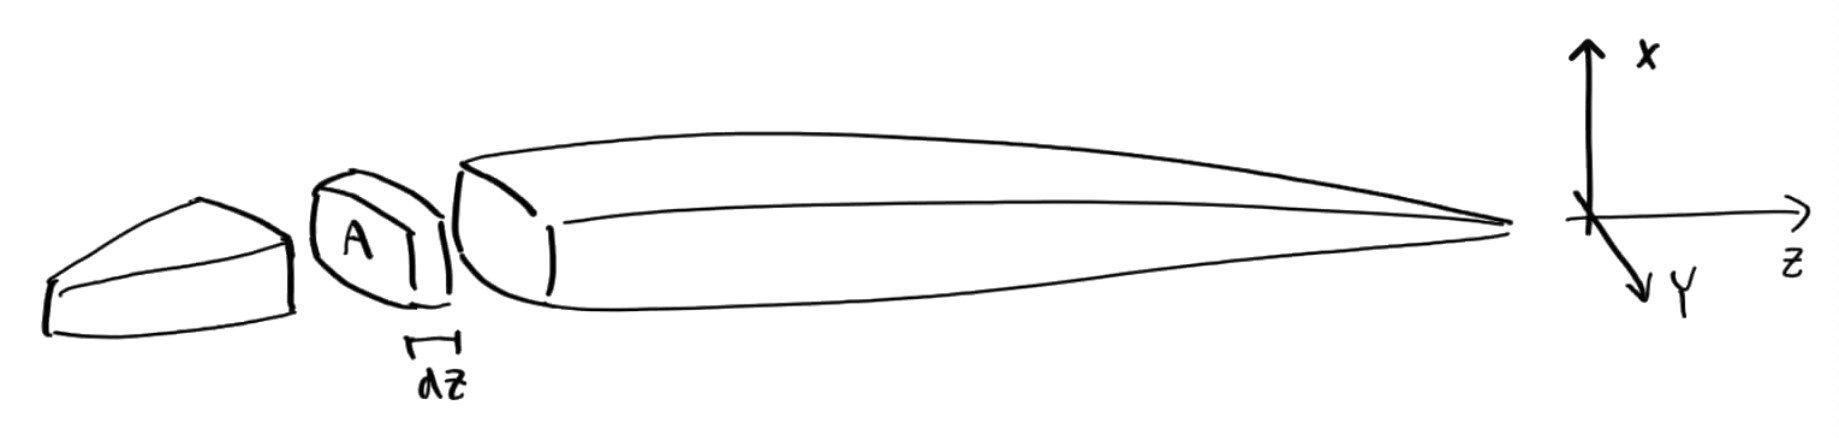
\includegraphics[scale=0.25]{Illustrations/BEMwingcut.jpg}
    \caption{Illustration of turbine blade cross section}
    \label{fig:bladeslice}
\end{figure}

In normal operation, we'll have 2 wind components, one for the incoming flow $U_\infty$ and one for the rotation $U_r$. The rotational wind component will naturally be in the tangential direction, while the incoming flow is angled by the yawing on the turbine. Such wind condition is illustrated on a blade slice in figure \ref{fig:winddirections}.

\begin{figure}[H]
    \centering
    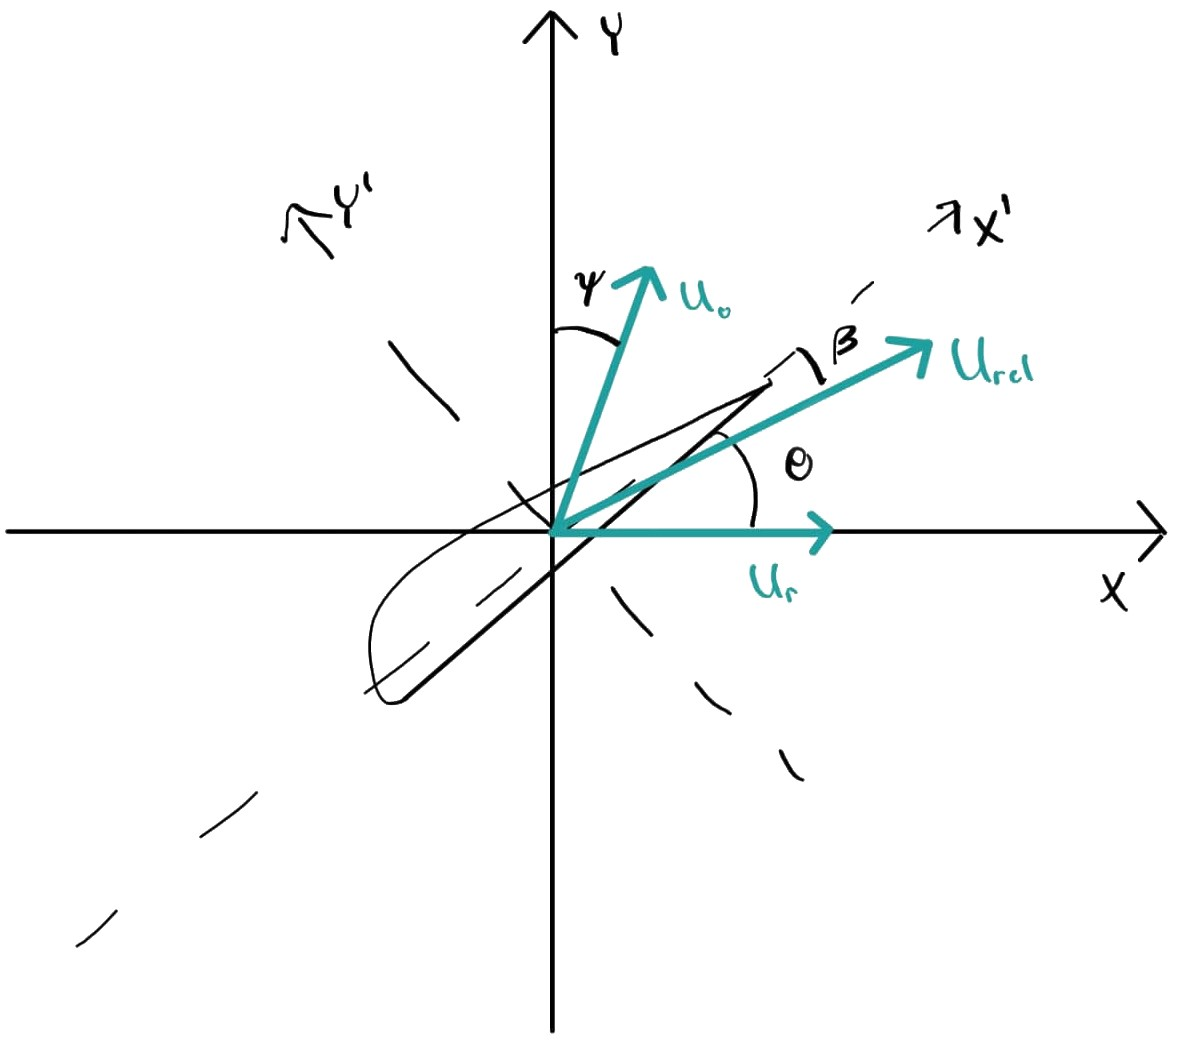
\includegraphics[scale=0.28]{Illustrations/BEMillustation1.jpg}
    \caption{Cross section with velocity components}
    \label{fig:winddirections}
\end{figure}

where $\psi$ is the yawing angle, $\theta$ is the pitching angle and $\beta$ is the angle between the relative velocity $U_{rel}$ and the local axis of the airfoil. The velocity acting on the blade will undoubtedly be lower than the free stream velocity due to the pressure drop after the energy is extracted. Likewise does the velocity, due to rotation, depend on which part of the blade we look at. To account for this, we'll introduce axial factors $\alpha$ and $\alpha^\prime$, and describe the velocities as

\begin{equation}
    U_0 = U_\infty (1-\alpha),
\end{equation}

\begin{equation}
    U_r = \Omega R (1-\alpha^\prime).
\end{equation}

Additionally, it should be mentioned that $\alpha^\prime$ could be expressed as $\alpha^\prime=\left( 1-\frac{z}{R} \right)$, since the velocity increases linearly across the length of the blade. With simple geometry, the magnitude of the relative velocity then becomes

\begin{equation}
    U_{rel} = \sqrt{\left(U_{\infty}(1-\alpha) \sin (\varphi)+\Omega R \left(1-\alpha^\prime\right)\right)^2+U_{\infty}(1-\alpha) \cos (\varphi)^2}.
\end{equation}

The pressure acting on the blade in each direction may be calculated as

\begin{equation}
    P_{x} = \frac{1}{2}\rho C_x(l,\beta,\phi) \cdot U_{rel}^2,
\end{equation}

\begin{equation}
    P_{y} = \frac{1}{2}\rho C_y(l,\beta,\phi) \cdot U_{rel}^2,
\end{equation}

where $C_x$ and $C_y$ are form factors, varying as a function of the angle of attack $\beta$, pitch $\phi$, and position on the blade $l$. It should also be mentioned that $\beta$ could be expressed by the velocity magnitudes, pitch, and yaw but is kept this way to keep expressions short. The total torque can then be summed up across the blade, which yields

\begin{equation}
    T_x=\int_0^LP_x(z) dA = P_x(z) \cdot h(z) dz,
\end{equation}

\begin{equation}
    T_y=\int_0^LP_y(z) dA = P_y(z) \cdot b(z) dz.
\end{equation}

For rotational bodies, power is generally defined as torque times rotational speed:

\begin{equation}
    \label{powerequation}
    P=\Omega \cdot T_x.
\end{equation}

Though Flex5 calculates other parameters from BEM, the derivation all share the same general idea. Since power and blade loads are most relevant for our analysis, the theory will be kept as is.

\subsection{Modal analysis}

BEM is useful for specific quantities but does not give insight into blade deflections. These can, however, be very important if the load fluctuates approach the natural frequency of the blades. In theory, this might cause immense deflections and stresses within the structure. To account for such situations, Modal analysis \cite{modal} can be applied to determine mode shapes and natural frequencies.

\\

Consider an elastic structure and its belonging displacement equation. Taking possible non-linearities into account, this might be described in a general sense as a partial differential equation. If one chose to separate linear and nonlinear terms, the relation could be written as

\begin{equation}
L[w]=g(w, \dot{\omega}, t),
\label{partialmodal}
\end{equation}

where $L$ is a differential operator, and $g$ is a function describing dampening and periodic loads. To solve such an equation, we will start by looking at the free undampened system, where $g=0$ and $w(x, t)=\varphi(x) \sin (\omega t)$. The differential eigenvalue problem then becomes:

\begin{equation}
L[w]=0.
\end{equation}

First we find the free natural frequencies $\omega=\omega_j$ and the connected oscillation modes $\varphi(x)=\varphi_j(x), j=1,2,...$. Like a Fourier series, $w$ then be described as an infinite sum of these

\begin{equation}
w(x, t)=\sum_{j=1}^N y_j(t) \varphi_j(x).
\label{modalsolution}
\end{equation}

Note that this approximation becomes exact for $N \rightarrow \infty$. Inserting this expression in \ref{partialmodal} and integrating over the length yields

\begin{equation}
\int_0^l \varphi_i(x) L\left[\sum_{j=1}^N y_j \varphi_j(x) \right] d x=\int_0^l \varphi_i(x) g\left(\sum_{j=1}^N y_j \varphi_j(x), \sum_{j=1}^N \dot{y}_j \varphi_j(x), t\right) d x .
\end{equation}

By simplification, this leads to $N$ ordinary differential equations, usually referred to as the modal equations. If the eigenvectors turn out to be orthogonal (which is often the case), this will lead to

\begin{equation}
\ddot{y}_j+\omega_j^2 y_j=p_j(\mathbf{y}, \dot{\mathbf{y}}, t), \quad j=1,2,..,N, \quad \mathbf{y}=\{y_1,y_2,..,y_N \}
\end{equation}

With $y_j$ being the modal factors. These factors can then be summed up by \ref{modalsolution}, giving us the deflection.

On a side note of the application of this theory for turbine blades, it should be mentioned that for transverse oscillations in beams, \ref{partialmodal} becomes

\begin{equation}
\frac{\partial^2 \omega}{\partial t^2} + \frac{E(x) I(x)}{\rho A(x)} \frac{\partial^4 \omega }{\partial x^4} = f(x, t)-c \dot{\omega}
\end{equation}

Solving this for the blades beforehand allows us to assume specific mode shapes and makes the actual calculations very fast. 

%%%%%%%%%%%%%%%%%%%%%%%%%%%%%%%%%%%%%%%%%%%%%%%%%%%%%%%%%%%%%%%%%%%%%%%%%%%%
\section{Surrogates}

Introductory statistics bring many methodologies for describing and predicting various data distributions. However, these mathematical models become increasingly complex when introducing additional variables and dependencies, and even more advanced multi-variable models sometimes struggle to describe these relations. Therefore one might imagine that the case of 2 turbines, where the power distribution can be affected by a single DOF, might be challenging to describe through common statistics. A way to tackle this is to go for a more empirical approach, where we will consider a random model, which we will tune to match our simulated data cases. This general line of thought is more commonly referred to as machine learning \cite{3blue1brown} and is an incredibly useful tool in such situations. More precisely, this thesis will utilize an elementary branch of machine learning called "Feedforward neural network", which is assumed to be adequate for the problem at hand.

\subsection{Feed forward neural network}

\subsubsection*{Definition}

Consider a simple case of x inputs and y outputs. In between these apparent quantities, we will introduce a network of $l$ layers and $n_i$ neurons per layer, as illustrated in figure \ref{fig:network}. A neuron is then defined as a scalar often restrained within a set range and determined as a function of the previous layers neurons.

\begin{figure}[H]
    \centering
    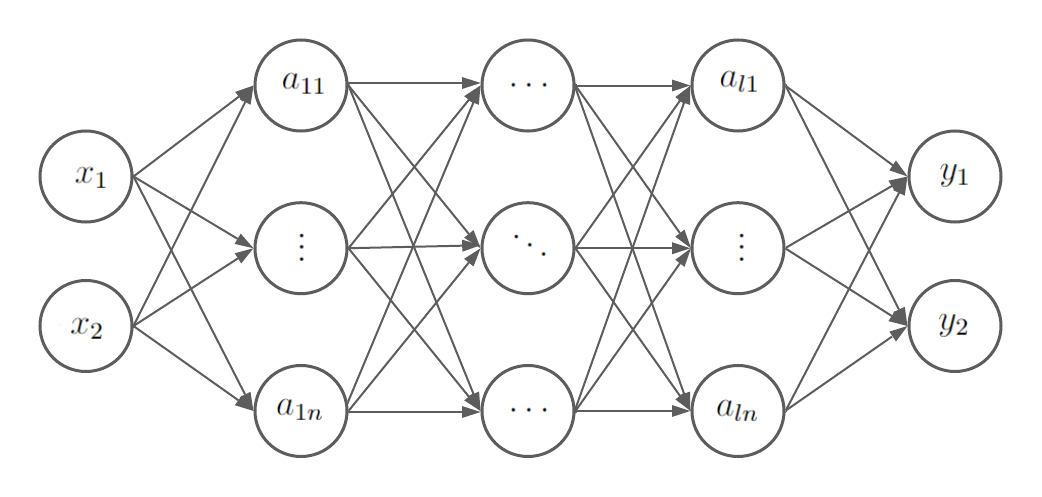
\includegraphics[scale=0.28]{Illustrations/neural.png}
    \caption{Illustration of neural network}
    \label{fig:network}
\end{figure}

More precisely, we will introduce an activation function to represent said scalar as a function of the previously determined scalars, all the way back to the input variables. There are many ways this might be done, but for the sake of simplicity, we will define the value of a single neuron linearly. The expression then becomes

\begin{equation}
    a_{l,n} = \sigma \left( w_{l,1} a_{(l-1),1} + w_{l,2} a_{(l-1),2} + \hdots + w_{l,N} a_{(l-1),N} + b_{l,n}\right),
    \label{activationfunction}
\end{equation}

where l and n are indexes representing layer and neuron respectively. $w_{l,n}$, also called the weight, is a value describing how much influence each previous neuron should have on the value, $b_{l,n}$ being an additional bias and $\sigma$ a function which squeezes the result to a value within the defined range. Such scaling could be expressed in multiple ways, the most common being the Sigmoid and ReLU functions \cite{activationfunction}. It should also be mentioned that the range is not random, but defined by the applied activation function. For Sigmoid this would be between 0 and 1. Additionally, the expression could be shortened by writing in matrix form:

\begin{equation}
\mathbf{a}_l=\sigma\left(\mathbf{W}_{l-1} \mathbf{a}_{l-1}+\mathbf{b}_{l}\right).
\end{equation}
 

\subsubsection*{Training}

In layman's terms, the "training" of a network could be described as the simple act of determining the best values for the beforehand mentioned weights and biases. The process, however, is not as elementary as one might expect. To describe how well the network is performing for a given set of weights, we define a cost function as the sum of squares between the predicted values and the right output.

\begin{equation}
C_L=\sum_{j=1}^{N_L}\left(a_{j,L}-y_j\right)^2.
\end{equation}

Since the weights and biases are the only parameters we can change, it is obvious to explore how these could be altered to minimize this function. This expression might be a little complicated due to all the compositions of different functions. We will, therefore, introduce a function beforehand to simplify the notation. 

\begin{equation}
z_{j,L}=w_{j 1,L} \cdot a_{1,(L-1)}+w_{j 2,L} \cdot a_{2,(L-1)}+ \hdots + w_{j N,L} \cdot a_{N,(L-1)}+b_{j,L},
\end{equation}

\begin{equation}
a_{j,L}=\sigma\left(z_{j,L}\right),
\end{equation}

with $j$ being a variable running over the number of neurons in each layer. With this simplification, the partial derivatives become

\begin{equation}
\frac{\partial C_L}{\partial w_{j k,L}}=\frac{\partial z_{j,L}}{\partial w_{j k,L}} \frac{\partial a_{j,L}}{\partial z_{j,L}} \frac{\partial C_L}{\partial a_{j,L}} = a_{k,(l-1)}\sigma^\prime (z_{j,l}) \frac{\partial C_L}{\partial a_{j,L}},
\end{equation}
\begin{equation}
\frac{\partial C_L}{\partial b_{j,L}}=\frac{\partial z_{j,L}}{\partial b_{j,L}} \frac{\partial a_{j,L}}{\partial z_{j,L}} \frac{\partial C_L}{\partial a_{j,L}} = \sigma^\prime (z_{j,l}) \frac{\partial C_L}{\partial a_{j,L}}.
\end{equation}

Note that the cost function partially derived with respect to the current neuron depends on how much that neuron contributes to the next layer, hence:

\begin{equation}
\frac{\partial C_L}{\partial a_{j,L}} = \sum_{h=1}^{N_{l+1}} w_{h k,(l+1)} \sigma^{\prime}\left(z_{h,(l+1)}\right) \frac{\partial C}{\partial a_{h,(l+1)}}.
\end{equation}


We can then adjust each variable according to its importance on the cost function. This method is known as gradient ascend and allows us to slowly approach a local minimum of the cost function. Though a local minimum is not necessarily the best possible configuration, finding the global minimum is way more complex and will not be discussed nor applied in this thesis. Obviously, this requires an enormous amount of calculations, which can take much computational time. A way to alleviate this is to only test a sample of the training data before adjusting the weights. Such sampling is referred to as a batch and works by approximating the gradient for the entire data set. Though it is technically less accurate, the run time is heavily decreased, resulting in less computational time.


\subsubsection*{Application}

In the case of 2 turbines, we want to predict a Weibull fit for the CDF power/load distribution depending on the configuration of the turbines. Therefore, in principle, we will have seven inputs, the three control parameters for each turbine and the spacing in between. We will, however, keep the analysis simple and let the control of the second turbine automatically determine pitch and rotational speed as it would normally. The spacing is likewise simplified by only looking at two distances. We will, as a result, only have four inputs and two outputs, with the inputs being the three control parameters for the first turbine and the outputs being the Weibull constants.

%%%%%%%%%%%%%%%%%%%%%%%%%%%%%%%%%%%%%%%%%%%%%%%%%%%%%%
\section{Fatigue calculations}

The output of flex5 results in a large array of load data, which due to the turbulent air, wildly fluctuates around a mean value, as illustrated in figure \ref{fig:flap_load_example}. 

\begin{figure}[H]
    \centering
    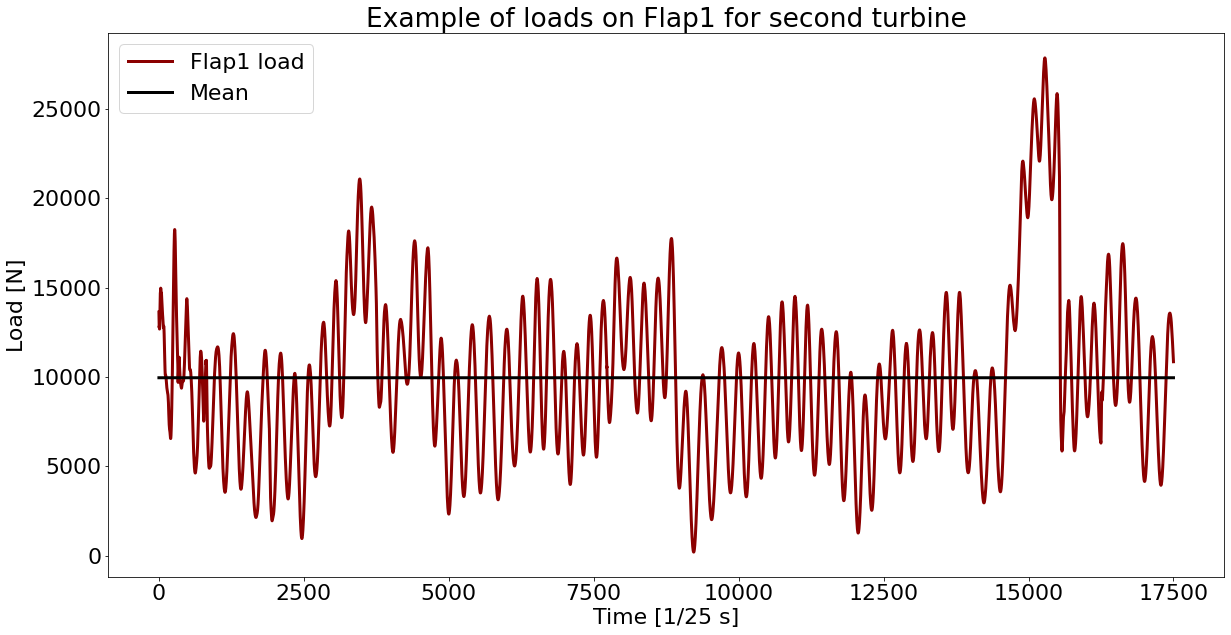
\includegraphics[scale=0.22]{Illustrations/flap_load_example.png}
    \caption{Example of load on flap for $\psi_1 = 20^\circ, \; \theta_1 = -0.5^\circ, \; \Omega_1 = 0.75 \frac{m}{s}, \; \psi_2 = 5^\circ$}
    \label{fig:flap_load_example}
\end{figure}

Generally, fatigue is evaluated from a periodic load with $n_i$ cycles of amplitude $S_i$, and each material has an empirical found value for cycles until failure $N_i$ at a given amplitude. By this logic, we can describe a damage factor as the percentage of the total fatigue the material has endured. 

\begin{equation}
d_i=\frac{n_i}{N_i}
\end{equation}

According to the Palmgren-Miner linear damage hypothesis, the relationship between amplitude and cycles to failure is linear in a log-log plot with a slope of $1/m$ \cite{fatiguelink}. The damage can then be described as

\begin{equation}
d_i=\frac{n_i S_i^m}{S_0^m},
\end{equation}

where $S_0$ is the amplitude at $N_i=0$ and $m$ is the Wöhler exponent. This exponent is, as previously mentioned, found by empirical experiments but can, for our use case, be roughly approximated as 5 for the tower and 10 for the blades. In the case of cycles at multiple amplitudes, the damage is summed up as

\begin{equation}
D=\sum d_i=\frac{1}{S_0^m} \sum n_i S_i^m
\end{equation}

Since we now have an expression for the total load over a time period, it might be useful to calculate the equivalent amplitude for a given number of cycles. Here we denote $n_{eq}$ as a chosen value for testing, in practice represented as a frequency over time, and $S_{eq}$ as the matching amplitude, which results in equal fatigue:

\begin{equation}
D=\frac{n_{e q} S_{e q}^m}{S_0^m}.
\end{equation}

Solving for the amplitude gives us

\begin{equation}
S_{e q}=\left(\frac{\sum n_i S_i^m}{n_{e q}}\right)^{\frac{1}{m}}.
\label{DEL}
\end{equation}

DEL is an instrumental figure since it can be used both as a practical way to test essential components and as an indicator of total damage. For our analysis, this will be used as the latter, where the damage equivalent load (DEL) will be compared between the different configurations.


\section{Rainflow counting}

DEL will be an essential measure of loads throughout the analysis, but it might be noted from equation \ref{DEL} that the data needs to be separated into periodic loads of equal amplitude. To simplify the raw data, we use the rain flow counting algorithm \cite{rainflowref}, which is the standard for such applications. The algorithm simplifies the data and then counts cycles of each amplitude. The process can, in broad terms, be described as 

\begin{enumerate}

  \item Round data points to a fitting accuracy.

  \item Remove data points outside peaks and valleys.

  \item Count half and full cycles between remaining data points. 

\end{enumerate}

This is, of course, a very vague description but gives a general idea of the process. The resulting cycle count can then be applied to \ref{DEL} to calculate the equivalent load. 

